\chapter{Generadores estudiados}
\label{cap:generadores}

En el capítulo anterior se vio que un LFSR aislado no sirve para criptografía,
ya que su complejidad lineal es igual a su grado y Berlekamp-Massey lo rompe con muy pocos bits.
La solución es combinar varios LFSR de formas distintas para que la secuencia resultante tenga una complejidad lineal mucho mayor.

En este capítulo se describen los cuatro generadores que se han implementado.
Cada uno usa una estrategia diferente. Geffe combina tres registros con una función booleana,
Shrinking descarta bits de forma selectiva, Self-Shrinking aplica la misma idea con un solo registro,
y ASG alterna el avance de dos registros controlados por un tercero.
Para cada uno se explica el mecanismo, se muestra el código real que lo implementa y se presenta una ejecución que mide la complejidad lineal alcanzada.

\section{Generador de Geffe}
\label{sec:geffe}

El generador de Geffe~\cite{geffe1973} fue una de las primeras propuestas para combinar LFSR de forma no lineal.
Usa tres registros $R_1$, $R_2$ y $R_3$ que avanzan a la vez en cada ciclo, y el bit de $R_1$ decide cuál de los otros dos se manda a la salida.

\[
  s_i = \begin{cases} b_i & \text{si } a_i = 1 \\ c_i & \text{si } a_i = 0 \end{cases}
\]

donde $a_i$, $b_i$, $c_i$ son los bits actuales de $R_1$, $R_2$ y $R_3$. Es básicamente un multiplexor 2 a 1 controlado por el primer registro.

\subsection{Ejemplo}

Para ver cómo funciona, usamos LFSR pequeños.

\begin{itemize}
  \item $R_1$, grado 3, polinomio $x^3 + x + 1$, estado inicial $(1, 0, 1)$.
  \item $R_2$, grado 4, polinomio $x^4 + x + 1$, estado inicial $(1, 1, 0, 0)$.
  \item $R_3$, grado 5, polinomio $x^5 + x^2 + 1$, estado inicial $(1, 0, 1, 1, 0)$.
\end{itemize}

\begin{center}
\begin{tabular}{c|ccc|c|l}
\hline
$t$ & $a$ ($R_1$) & $b$ ($R_2$) & $c$ ($R_3$) & $s$ & Selección \\
\hline
1 & 1 & 0 & 0 & 0 & $a=1 \Rightarrow s = b$ \\
2 & 0 & 0 & 1 & 1 & $a=0 \Rightarrow s = c$ \\
3 & 1 & 1 & 1 & 1 & $a=1 \Rightarrow s = b$ \\
4 & 1 & 1 & 0 & 1 & $a=1 \Rightarrow s = b$ \\
5 & 0 & 0 & 1 & 1 & $a=0 \Rightarrow s = c$ \\
6 & 1 & 1 & 1 & 1 & $a=1 \Rightarrow s = b$ \\
7 & 0 & 0 & 0 & 0 & $a=0 \Rightarrow s = c$ \\
8 & 1 & 0 & 0 & 0 & $a=1 \Rightarrow s = b$ \\
\hline
\end{tabular}
\end{center}

La salida es $\{0, 1, 1, 1, 1, 1, 0, 0, \ldots\}$.
Cada bit resultante viene de $R_2$ o de $R_3$ según lo que diga $R_1$ en ese instante.

\subsection{Implementación}

\begin{lstlisting}[style=Python,caption={Generador de Geffe (\texttt{src/generators/geffe.py}).}]
def geffe_generator(r1: LFSR, r2: LFSR, r3: LFSR, n: int) -> list[int]:
    """Generates n bits using the Geffe generator."""
    output = []
    for _ in range(n):
        a = r1.next_bit()
        b = r2.next_bit()
        c = r3.next_bit()
        output.append((a & b) ^ ((1 ^ a) & c))
    return output
\end{lstlisting}

La función booleana equivalente es $(a \wedge b) \oplus (\neg a \wedge c)$, que es la forma estándar de un multiplexor.

\subsection{Complejidad lineal}

Ejecutamos el generador con los polinomios $R_1$ de grado 7, $R_2$ de grado 5 y $R_3$ de grado 9 (todos primitivos),
sobre una secuencia de 1000 bits, midiendo la complejidad lineal con Berlekamp-Massey.

\begin{figure}[H]
\centering
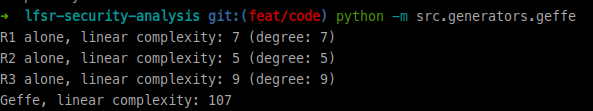
\includegraphics[width=0.9\textwidth]{images/execution_geffe.png}
\caption{Salida de \texttt{python -m src.generators.geffe}.}
\label{fig:exec-geffe}
\end{figure}

La complejidad lineal pasa de los grados originales (7, 5, 9) a 107. Hay una mejora clara, pero como veremos a continuación,
la complejidad lineal alta no salva al generador.

\subsection{La debilidad real, correlación}

El problema del generador de Geffe no es la complejidad lineal sino la correlación entre la salida y los LFSR internos.
Si miramos cuántas veces coincide la salida $s$ con $R_2$,

\[
  \Pr[s = b] = \Pr[s = b \mid a = 1]\Pr[a = 1] + \Pr[s = b \mid a = 0]\Pr[a = 0]
  = 1 \cdot \tfrac{1}{2} + \tfrac{1}{2} \cdot \tfrac{1}{2} = \tfrac{3}{4}
\]

La salida coincide con $R_2$ el 75\% de las veces. Lo mismo pasa con $R_3$.
Un atacante con un fragmento de keystream puede probar todos los estados posibles de $R_2$
(solo $2^5 = 32$ para nuestro ejemplo) y quedarse con el que produce coincidencia $\sim 75\%$.
Repite con $R_3$ y deduce $R_1$ a partir de los dos.

El coste total pasa de $2^{n_1 + n_2 + n_3}$ (fuerza bruta completa) a $2^{n_1} + 2^{n_2} + 2^{n_3}$, mucho menor.
Para nuestros tamaños son $2^7 + 2^5 + 2^9 = 672$ operaciones frente a $2^{21} \approx 2$ millones.
Y la correlación de $0{,}75$ no depende del tamaño de los registros, así que da igual usar LFSR de grado 100,
la vulnerabilidad sigue ahí.

Por esta razón el generador de Geffe se rompió conceptualmente con los ataques de correlación
de Siegenthaler~\cite{siegenthaler1985} y hoy no se usaría en producción.
En este trabajo sirve como caso base, ya que es el ejemplo perfecto de
que una complejidad lineal alta no basta si la función de combinación tiene correlación con sus entradas.

\section{Generador Shrinking}
\label{sec:shrinking}

El generador Shrinking, propuesto por Coppersmith, Krawczyk y Mansour~\cite{coppersmith1993}, funciona de forma completamente distinta a Geffe.
En vez de combinar las salidas con una función booleana, usa un registro para decidir qué bits del otro se incluyen en la salida y cuáles se tiran.

Los dos LFSR avanzan a la vez en cada ciclo,

\[
  s_i = \begin{cases} b_i & \text{si } a_i = 1 \\ \text{se descarta} & \text{si } a_i = 0 \end{cases}
\]

La consecuencia importante es que la secuencia de salida pierde la relación temporal con el reloj interno.
Un atacante que observe la secuencia no sabe cuántos ciclos han pasado entre dos bits consecutivos,
ya que no sabe cuántos se descartaron por el camino. Esto es lo que hace tan difícil aplicar Berlekamp-Massey directamente,
la secuencia que ve el atacante no es la salida directa de ningún LFSR, sino un muestreo irregular de uno.

\subsection{Ejemplo}

\begin{itemize}
  \item $R_1$ (selector), grado 3, polinomio $x^3 + x + 1$, estado $(1, 0, 1)$.
  \item $R_2$ (datos), grado 4, polinomio $x^4 + x + 1$, estado $(1, 1, 0, 0)$.
\end{itemize}

\begin{center}
\begin{tabular}{c|cc|c|l}
\hline
$t$ & $a$ ($R_1$) & $b$ ($R_2$) & Salida & Acción \\
\hline
1 & 1 & 0 & 0 & $a=1$, incluir $b$ \\
2 & 0 & 0 & --- & $a=0$, descartar \\
3 & 1 & 1 & 1 & $a=1$, incluir $b$ \\
4 & 1 & 1 & 1 & $a=1$, incluir $b$ \\
5 & 0 & 0 & --- & $a=0$, descartar \\
6 & 1 & 1 & 1 & $a=1$, incluir $b$ \\
7 & 0 & 0 & --- & $a=0$, descartar \\
8 & 1 & 0 & 0 & $a=1$, incluir $b$ \\
\hline
\end{tabular}
\end{center}

De 8 ciclos salen 5 bits, $\{0, 1, 1, 1, 0\}$.
Como $R_1$ produce aproximadamente la mitad de unos, de media se necesitan 2 ciclos por bit de salida.

\subsection{Implementación}

\begin{lstlisting}[style=Python,caption={Generador Shrinking (\texttt{src/generators/shrinking.py}).}]
def shrinking_generator(r1: LFSR, r2: LFSR, n: int) -> list[int]:
    """Generates n bits. r1 filters the output of r2."""
    output = []
    max_clocks = n * 10
    clocked = 0

    while len(output) < n and clocked < max_clocks:
        a = r1.next_bit()
        b = r2.next_bit()
        clocked += 1
        if a == 1:
            output.append(b)

    if len(output) < n:
        raise RuntimeError(
            f"could not generate {n} bits after {max_clocks} clocks"
        )

    return output
\end{lstlisting}

El parámetro \texttt{max\_clocks} es una protección, si por algún motivo $R_1$ produjera demasiados ceros consecutivos,
el bucle terminaría con un error en vez de quedarse colgado.

\subsection{Complejidad lineal}

Ejecutamos el generador con los mismos parámetros que antes,
$R_1$ grado 7 y $R_2$ grado 5, generando 1000 bits.

\begin{figure}[H]
\centering
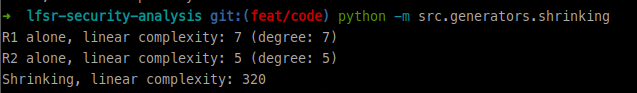
\includegraphics[width=0.9\textwidth]{images/execution_shrinking.png}
\caption{Salida de \texttt{python -m src.generators.shrinking}.}
\label{fig:exec-shrinking}
\end{figure}

El salto es espectacular. De LFSR de grados 7 y 5 (que individualmente tendrían complejidad lineal 7 y 5),
salimos con una complejidad lineal de 320. El factor de mejora frente al LFSR más grande es de unos 45x.
Y a diferencia de Geffe, no hay correlación directa explotable, ya que un atacante no sabe en qué posición del ciclo de $R_2$ está cada bit de la salida.

\subsection{Consideraciones prácticas}

La debilidad principal del Shrinking es que la seguridad depende de que $R_1$ sea desconocido.
Si alguien adivinara la secuencia de selección, sabría qué bits de $R_2$ forman la salida y aplicaría Berlekamp-Massey directamente.
El coste de esa fuerza bruta es $2^{n_1}$, así que se recomienda usar $n_1$ de al menos 64 bits en aplicaciones reales.

La otra consideración es la tasa de generación, no es constante, ya que cada bit de salida cuesta de media 2 ciclos de reloj.
En software esto no importa, basta llamar al generador en un bucle hasta tener los bits necesarios.
En hardware sí complica el diseño, hay que añadir un buffer entre el generador y el dispositivo que consume los bits para mantener una tasa de salida fija.

\section{Generador Self-Shrinking}
\label{sec:self-shrinking}

El Self-Shrinking, propuesto por Meier y Staffelbach~\cite{meier1994}, es una variante del Shrinking que usa un solo LFSR.
La idea es la misma (selección irregular) pero aplicada sobre la propia secuencia del registro.

Se toman los bits del LFSR de dos en dos. En cada par $(a, b)$, si $a = 1$ el bit $b$ pasa a la salida,
y si $a = 0$ se descartan los dos. La ventaja es que solo hace falta un registro.
La desventaja es que la tasa baja a un bit cada 4 ciclos (cada par consume 2 ciclos y solo la mitad de los pares producen salida).

\subsection{Ejemplo}

Un LFSR de grado 4 con polinomio $x^4 + x + 1$ y estado $(1, 1, 0, 0)$.

\begin{center}
\begin{tabular}{c|cc|c|l}
\hline
Par & $a$ & $b$ & Salida & Acción \\
\hline
1 & 0 & 0 & --- & $a=0$, descartar \\
2 & 1 & 1 & 1 & $a=1$, incluir $b$ \\
3 & 0 & 0 & --- & $a=0$, descartar \\
4 & 1 & 1 & 1 & $a=1$, incluir $b$ \\
5 & 0 & 1 & --- & $a=0$, descartar \\
6 & 0 & 0 & --- & $a=0$, descartar \\
7 & 1 & 0 & 0 & $a=1$, incluir $b$ \\
8 & 1 & 0 & 0 & $a=1$, incluir $b$ \\
\hline
\end{tabular}
\end{center}

16 bits del LFSR (8 pares) dan 4 bits de salida, $\{1, 1, 0, 0\}$.

\subsection{Implementación}

\begin{lstlisting}[style=Python,caption={Generador Self-Shrinking (\texttt{src/generators/self\_shrinking.py}).}]
def self_shrinking_generator(r: LFSR, n: int) -> list[int]:
    """Generates n bits from a single LFSR using self-shrinking."""
    output = []
    max_clocks = n * 10
    clocked = 0

    while len(output) < n and clocked < max_clocks:
        a = r.next_bit()
        b = r.next_bit()
        clocked += 2
        if a == 1:
            output.append(b)

    if len(output) < n:
        raise RuntimeError(
            f"could not generate {n} bits after {max_clocks} clocks"
        )

    return output
\end{lstlisting}

\subsection{Complejidad lineal}

Ejecutamos sobre un LFSR de grado 11 con polinomio $x^{11} + x^2 + 1$, generando 1000 bits.

\begin{figure}[H]
\centering
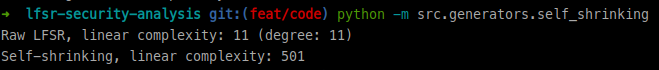
\includegraphics[width=0.9\textwidth]{images/execution_self_shrinking.png}
\caption{Salida de \texttt{python -m src.generators.self\_shrinking}.}
\label{fig:exec-self-shrinking}
\end{figure}

De nuevo el salto es enorme, de 11 a 501, factor 45x. La complejidad lineal queda en valores similares al Shrinking con menos hardware.

\subsection{Diferencias con el Shrinking}

Aunque el mecanismo de fondo es el mismo, hay una diferencia importante.
En Shrinking, el selector ($R_1$) y los datos ($R_2$) son LFSR completamente independientes, con polinomios y estados distintos.
En Self-Shrinking los bits de selección y los bits de datos son bits consecutivos del mismo LFSR,
así que están relacionados por la recurrencia del registro.
Es una debilidad teórica, difícil de explotar en la práctica pero que existe.
Por eso para el mismo nivel de seguridad se recomienda usar un LFSR de mayor grado que en Shrinking.

\section{Alternating Step Generator (ASG)}
\label{sec:asg}

El ASG fue propuesto por Günther~\cite{gunther1987} y es el más elaborado de los cuatro generadores.
Usa tres LFSR como Geffe, pero la forma de combinarlos es muy distinta.

En cada ciclo se avanza el registro de control $R_1$ y se lee su bit de salida.
Si es 1 se avanza $R_2$ (y $R_3$ se queda quieto), y si es 0 se avanza $R_3$ (y $R_2$ se queda quieto).
La salida del generador es el XOR de los bits actuales de $R_2$ y $R_3$, independientemente de cuál haya avanzado en ese ciclo.

\[
  s_i = b_2 \oplus b_3
\]

donde $b_2$ y $b_3$ son los bits más recientes de $R_2$ y $R_3$.

Es interesante comparar esto con Geffe, ya que ambos usan tres LFSR pero con resultados muy distintos.
En Geffe los tres registros avanzan siempre, y la salida depende directamente de cada uno en cada instante.
Eso es lo que permite la correlación. En ASG, $R_2$ y $R_3$ no avanzan a la vez, sino que uno se queda parado mientras el otro avanza,
y la decisión la toma $R_1$. Esto rompe la sincronización temporal entre la salida y cada registro individual.
Además la salida es el XOR de ambos (no una selección), lo que mezcla las dos secuencias de forma más profunda.

\subsection{Ejemplo}

\begin{itemize}
  \item $R_1$ (control), grado 3, polinomio $x^3 + x + 1$, estado $(1, 0, 1)$.
  \item $R_2$, grado 4, polinomio $x^4 + x + 1$, estado $(1, 1, 0, 0)$.
  \item $R_3$, grado 5, polinomio $x^5 + x^2 + 1$, estado $(1, 0, 1, 1, 0)$.
\end{itemize}

Al inicio se extraen los primeros bits de $R_2$ y $R_3$, $b_2 = 0$ y $b_3 = 0$.

\begin{center}
\begin{tabular}{c|c|cc|c|l}
\hline
$t$ & $a$ ($R_1$) & $b_2$ & $b_3$ & $s = b_2 \oplus b_3$ & Acción \\
\hline
1 & 1 & 0 & 0 & 0 & Avanza $R_2$, $b_2 \leftarrow 0$ \\
2 & 0 & 0 & 0 & 1 & Avanza $R_3$, $b_3 \leftarrow 1$ \\
3 & 1 & 0 & 1 & 0 & Avanza $R_2$, $b_2 \leftarrow 1$ \\
4 & 1 & 1 & 1 & 0 & Avanza $R_2$, $b_2 \leftarrow 1$ \\
5 & 0 & 1 & 1 & 1 & Avanza $R_3$, $b_3 \leftarrow 0$ \\
6 & 1 & 1 & 0 & 0 & Avanza $R_2$, $b_2 \leftarrow 0$ \\
7 & 0 & 0 & 0 & 1 & Avanza $R_3$, $b_3 \leftarrow 1$ \\
8 & 1 & 0 & 1 & 1 & Avanza $R_2$, $b_2 \leftarrow 0$ \\
\hline
\end{tabular}
\end{center}

La salida es $\{0, 1, 0, 0, 1, 0, 1, 1, \ldots\}$.

\subsection{Implementación}

\begin{lstlisting}[style=Python,caption={Generador ASG (\texttt{src/generators/alternating\_step.py}).}]
def alternating_step_generator(r1: LFSR, r2: LFSR, r3: LFSR, n: int) -> list[int]:
    """Generates n bits. r1 decides which of r2/r3 advances."""
    output = []

    b2 = r2.next_bit()
    b3 = r3.next_bit()

    for _ in range(n):
        a = r1.next_bit()
        if a == 1:
            b2 = r2.next_bit()
        else:
            b3 = r3.next_bit()
        output.append(b2 ^ b3)

    return output
\end{lstlisting}

Una sutileza, los bits $b_2$ y $b_3$ se inicializan fuera del bucle. Esto es necesario porque en cada iteración solo se avanza uno de los dos,
así que el otro tiene que tener un valor previo válido para entrar en el XOR.

\subsection{Complejidad lineal}

Ejecutamos el generador con los mismos LFSR que usamos en Geffe,
grados 7, 5 y 9 con 1000 bits de salida.

\begin{figure}[H]
\centering
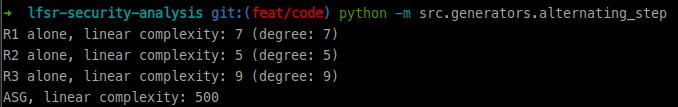
\includegraphics[width=0.9\textwidth]{images/execution_alternating_step.png}
\caption{Salida de \texttt{python -m src.generators.alternating\_step}.}
\label{fig:exec-asg}
\end{figure}

Esto es lo más interesante de todo el capítulo. Con los mismos LFSR que dieron 107 de complejidad lineal en Geffe,
el ASG llega a 500. La diferencia no está en los registros ni en sus tamaños sino exclusivamente
en cómo se combinan sus salidas. Reloj alterno y XOR de fuentes independientes amplifica mucho más la complejidad lineal que un multiplexor.

\subsection{Seguridad}

El ASG combina dos defensas a la vez, reloj irregular (un atacante no sabe cuántas veces avanzó cada registro)
y XOR de dos fuentes (aunque supiera el control $R_1$, todavía tendría que romper $R_2$ y $R_3$ a la vez).
No se conocen ataques de correlación prácticos cuando los registros son lo bastante grandes.

El mejor ataque conocido tiene coste del orden de $2^{n_2 + n_3}$,
fuerza bruta sobre los dos registros de datos en paralelo.
Con $n_2$ y $n_3$ de 64 bits cada uno, el ataque tiene coste $2^{128}$, que se considera fuera del alcance computacional actual.

\section{Resumen comparativo}

La tabla siguiente compara los cuatro generadores con los parámetros que vamos a usar en el análisis experimental del capítulo siguiente.

\begin{center}
\begin{tabular}{l|cccc}
\hline
& Geffe & Shrinking & Self-Shrinking & ASG \\
\hline
LFSR usados & 3 & 2 & 1 & 3 \\
Mecanismo & Multiplexor & Selección & Auto-selección & Reloj alterno \\
Ciclos por bit & 1 & $\sim 2$ & $\sim 4$ & 1 \\
LC sobre 1000 bits & 107 & 320 & 501 & 500 \\
Correlación con LFSR & 0,75 & No directa & No directa & No directa \\
\hline
\end{tabular}
\end{center}

Tres observaciones rápidas.

Primero, Geffe es el caso débil. Su complejidad lineal es menor que la de los otros tres (un orden de magnitud por debajo) y además tiene correlación 0,75,
lo que permite ataques mucho más eficientes que Berlekamp-Massey.

Segundo, Shrinking, Self-Shrinking y ASG quedan en complejidades lineales parecidas (320, 501, 500) con secuencias de 1000 bits.
En el capítulo siguiente, con secuencias más largas, se sigue manteniendo esta proximidad y los tres se acercan a $N/2$.

Tercero, comparando Geffe y ASG (que usan los mismos tres LFSR), la diferencia entre 107 y 500 sale solo del mecanismo de combinación.
Mismo hardware, conexión distinta, resultado completamente distinto. Esto es probablemente la lección más importante del trabajo,
en generadores basados en LFSR la clave no es el tamaño de los registros sino cómo se combinan.

El capítulo siguiente lleva todo esto un paso más allá, ejecuta los cuatro generadores con secuencias más largas, mide su complejidad lineal exacta
y los pasa por ocho tests estadísticos del estándar NIST para ver qué generador tiene la mejor calidad de salida en la práctica.
